\documentclass{zjureport}
% =============================================
% Part 1 Edit the info
% =============================================

\newcommand{\major}{大数据81}
\newcommand{\name}{林可可}
\newcommand{\stuid}{2183521635}
\newcommand{\newdate}{2021-07-11}


\newcommand{\course}{机器学习II}
\newcommand{\tutor}{Hao}
\newcommand{\grades}{59}
\newcommand{\newtitle}{机器学习II-大作业}
\newcommand{\exptype}{设计实验}
\newcommand{\group}{None}
\usepackage{listings}
\usepackage{ctex}
\usepackage{xcolor}
\usepackage{subfigure}
\usepackage{color}
\usepackage{graphics}
\usepackage{makecell}
\usepackage{booktabs}
\usepackage{caption2}
\usepackage{float}
\usepackage[noend]{algpseudocode}
\usepackage{algorithmicx,algorithm}

% 用来设置附录中代码的样式

\lstset{
    basicstyle          =   \sffamily,          % 基本代码风格
    keywordstyle        =   \bfseries,          % 关键字风格
    commentstyle        =   \rmfamily\itshape,  % 注释的风格,斜体
    stringstyle         =   \ttfamily,  % 字符串风格
    flexiblecolumns,                % 别问为什么,加上这个
    numbers             =   left,   % 行号的位置在左边
    showspaces          =   false,  % 是否显示空格,显示了有点乱,所以不现实了
    numberstyle         =   \zihao{-5}\ttfamily,    % 行号的样式,小五号,tt等宽字体
    showstringspaces    =   false,
    captionpos          =   t,      % 这段代码的名字所呈现的位置,t指的是top上面
    frame               =   lrtb,   % 显示边框
}

\lstdefinestyle{Python}{
    language        =   Python, % 语言选Python
    basicstyle      =   \zihao{-5}\ttfamily,
    numberstyle     =   \zihao{-5}\ttfamily,
    keywordstyle    =   \color{blue},
    keywordstyle    =   [2] \color{teal},
    stringstyle     =   \color{magenta},
    commentstyle    =   \color{red}\ttfamily,
    breaklines      =   true,   % 自动换行,建议不要写太长的行
    columns         =   fixed,  % 如果不加这一句,字间距就不固定,很丑,必须加
    basewidth       =   0.5em,
}


% =============================================
% Part 1 Main document
% =============================================
\begin{document}
\thispagestyle{empty}

\begin{titlepage}

\begin{center}

% Upper part of the page

\includegraphics[width=0.8\textwidth]{./head.png}\\[1.0cm]    

{\huge 机器学习II大作业}\\[1.0cm]


% Title

{ \huge Give Me Some Credit}\\[6.5cm]


\textsc{\Large 姓名:林可可}\\[0.35cm]

\textsc{\Large 学号:2183521635}\\[0.35cm]

\textsc{\Large 课程名称:机器学习II}\\[0.35cm]

\textsc{\Large 指导老师:林绍波}


\vfill

% Bottom of the page
{\large \today}

\end{center}

\end{titlepage}

\renewcommand{\contentsname}{目录}
\tableofcontents

\clearpage


\begin{center}
 \begin{tabular}{cccc}
    课程名称: & \underline\course   & 指导老师: & 林绍波\\
    实验名称: & \underline\newtitle & 实验类型: & 大作业
\end{tabular}
\end{center}




% =============================================
% Part 2 Main document
% =============================================

\section{实验目的和要求}
  通过自选数据集完成数据清洗与数据描述性分析,并寻找最少三个算法处理该数据并说明优劣,而后撰写数据分析报告。
\section{实验内容和步骤}

  \subsection{实验内容}

    首先对数据的背景以及研究意义进行阐述,而后进行数据的描述性统计,再对不同的算法进行对比,而后分析数据结果。

  \subsection{实验步骤}
    \begin{clause}
      \item Introduction:说明数据的背景及研究意义
      \item 描述性分析:说明对数据的直观感觉
      \item 算法描述:对不同的算法,优缺点进行描述并对比
      \item 数据分析结果
      \item 结论
    \end{clause}

\section{研究背景及意义}
\subsection{背景介绍}
本次大作业使用的数据集来自kaggle的公开数据集,Give Me Some Credit. 该数据集提供了贷款人的信用卡以及个人信贷的相关情况,包括每月的收入,开放信贷的数量和信用额度等相关指标。在了解这些指标之后,我们可以通过构建信用评分算法对贷款人违约概率进行预测,从而辅助银行进行是否应授予贷款的决策。 
\subsection{研究意义}
银行在市场经济中发挥着至关重要的作用。他们决定谁可以获得资金以及以什么条件获得资金,并且可以做出进行或终止投资的决策。为了让市场和社会的运作,个人和公司需要获得信贷。

考虑到数据集中提供了“个人经历了逾期90天的拖欠或者更糟糕的情况”(SeriousDlqin2yrs)这一指标,我们可以采取最先进的信用评分算法,通过预测某人在未来两年内遇到财务困境的可能性,
来支持借款人做出最佳财务决策。

\section{描述性统计}
\subsection{整体性描述}
首先对数据进行整体的查看。Kaggle提供的文件Data Dictionary.xls 包含了每一列的基本信息以及相关的示意,通过查看发现一共有十一列,其中第一列是样本的标签也即上文提到的“SeriousDlqin2yrs”,其余十列为样本的其他属性。
    %%image1-----------------(columns
    \begin{figure}[H]
    \centering
    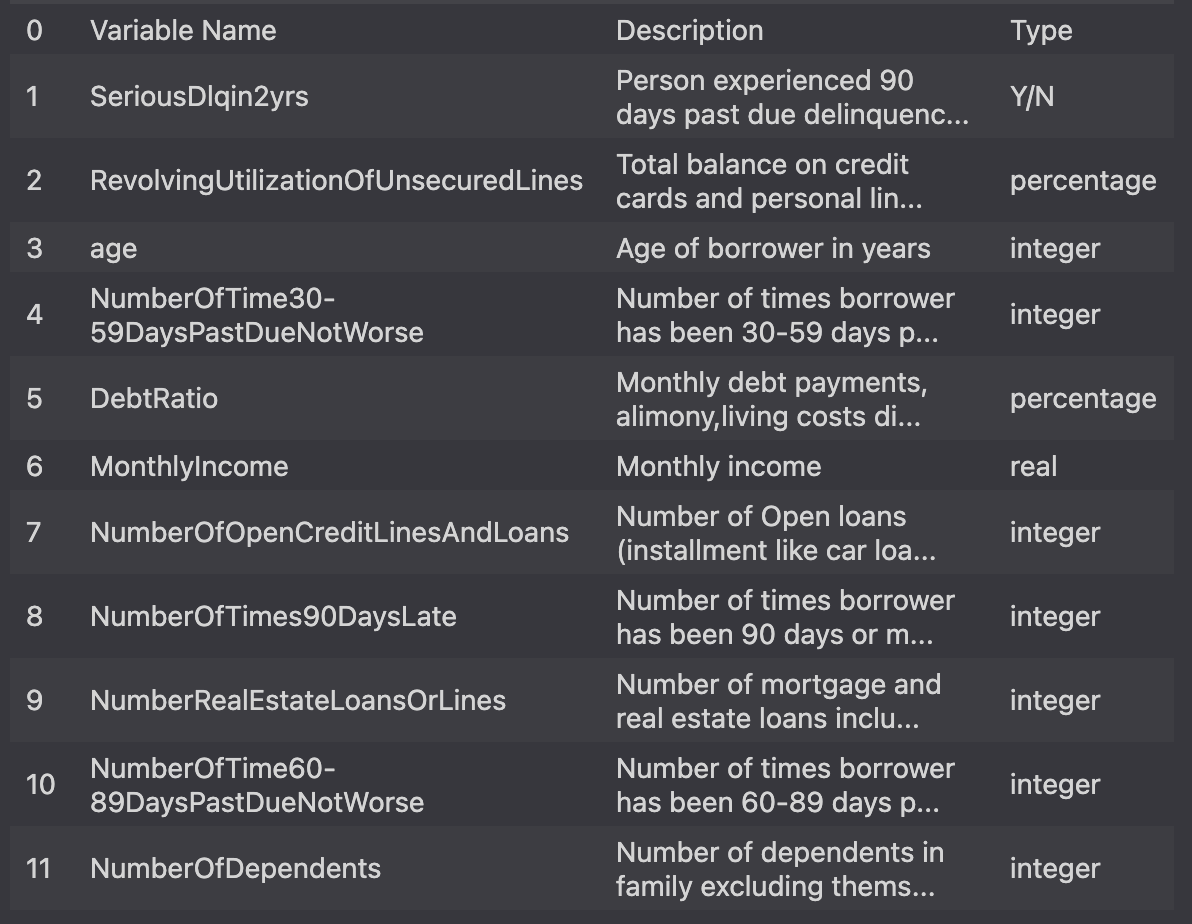
\includegraphics[scale=0.8]{figures/image1.png}\\
    \caption{数据概述}
    \end{figure}
    
    而后分别对训练集以及测试集的样本的大小进行查看,结果如下所示,其中训练集共有150000条样本,每个样本有11列属性(第一列为样本的顺序),同样的,测试集共有101503条样本,每个样本也是11列属性。
    %%image2-----------------(train.shape&test.shape)

    
    \begin{figure}[H]
    \centering  %图片全局居中
    \subfigure[训练集大小]{
    \label{Fig.sub.1}
    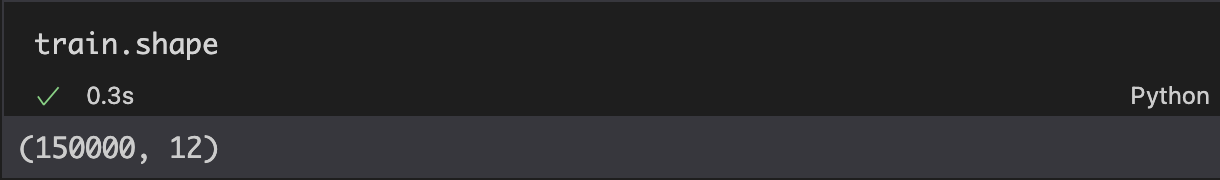
\includegraphics[width=0.45\textwidth]{figures/image2-1.png}}
    \subfigure[测试集大小]{
    \label{Fig.sub.2}
    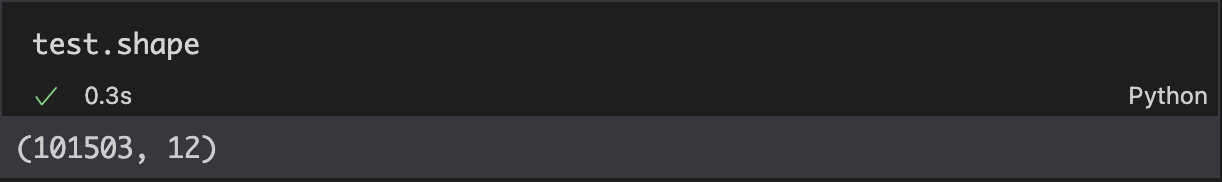
\includegraphics[width=0.45\textwidth]{figures/image2-2.png}}
    \caption{数据集大小}
    \label{Fig.main}
    \end{figure}


    
\subsection{分属性描述}
\begin{clause}
    \item SeriousDlqin2yrs表示个人经历了逾期90天的拖欠或者更糟糕的情况,通过简单的对比条形图我们可以发现该属性有明显的类别不均衡现象,通过进一步统计具体的数值我们知道其中标签为0的样本个数有139974个,而标签为1的样本仅有10026个。
    %%image3-----------------(分组条形图)
    \begin{figure}[H]
    \centering
    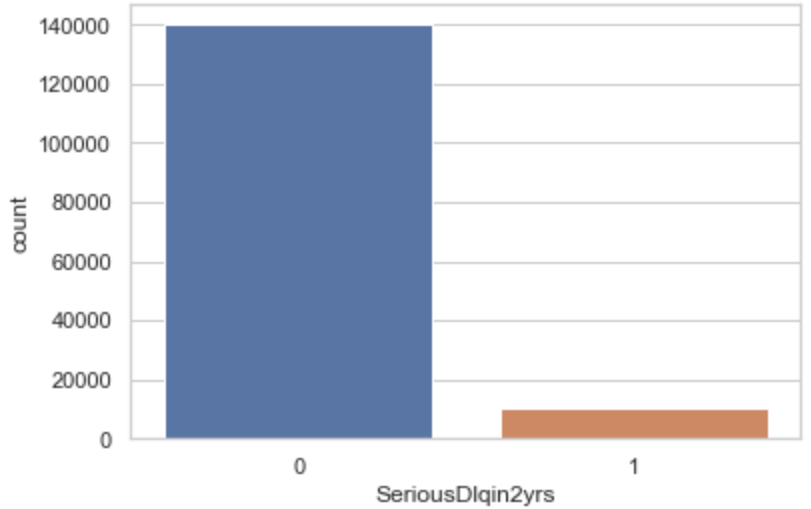
\includegraphics[scale=0.7]{figures/image3.png}\\
    \caption{SeriousDlqin2yrs分组条形图}
    \end{figure}
    \item RevolvingUtilizationOfUnsecuredLines表示信用卡和个人信贷的总余额,通过箱线图我们发现,该属性各个值之间的差异较大。
    %%image4-----------------(boxplot)
    \begin{figure}[H]
    \centering
    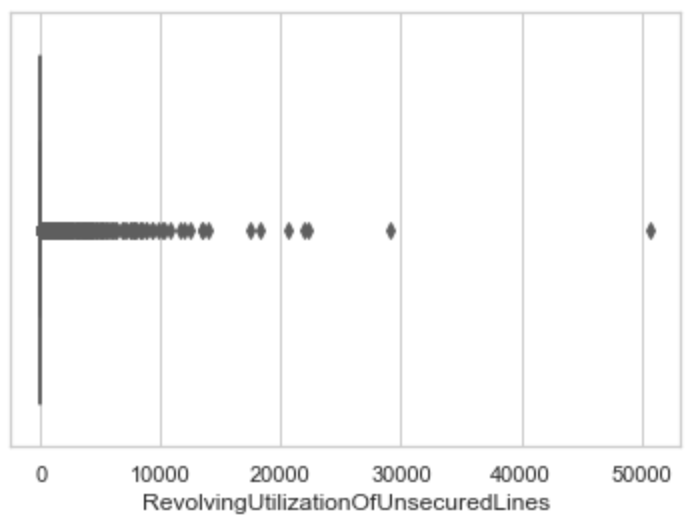
\includegraphics[scale=0.7]{figures/image4.png}\\
    \caption{RevolvingUtilizationOfUnsecuredLines箱线图}
    \end{figure}
    \item age表示贷款者的年龄,我们通过绘制直方图发现贷款者的年龄分布较为集中,其中40-60岁为贷款者年龄分布较多的区间,而后我们再次绘制了箱线图,发现确实是这样,落在箱线图区间外的outliers较少,年龄分布较为集中。而后我们结合SeriousDlqin2yrs绘制了分组箱线图,发现在两个类别下的贷款者年龄分布都比较集中,而没有逾期贷款的贷款者年龄稍微大一些略大于50岁,而有逾期贷款的贷款者的平均年龄略小于50岁,并且没有逾期贷款的贷款者年龄大于100岁的人数较多。
    %%image5-----------------(displot&boxplot&对比boxplot)
    \begin{figure}[H]
    \centering  %图片全局居中
    \subfigure[直方图]{
    \label{Fig.sub.1}
    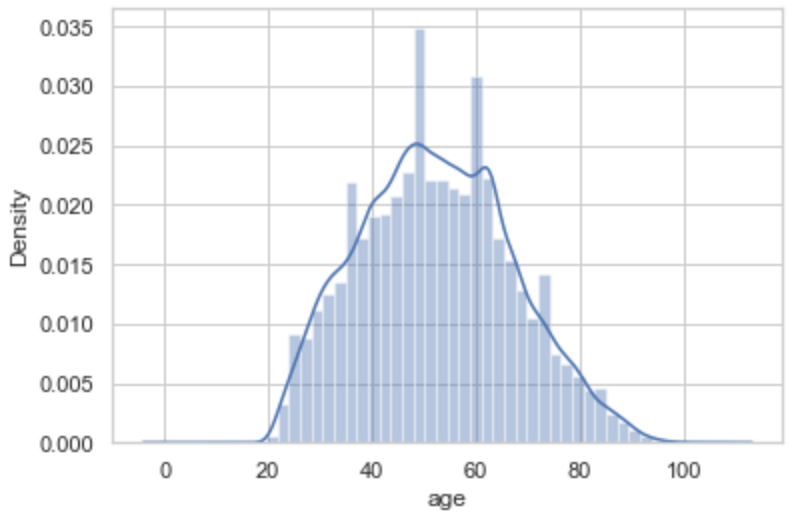
\includegraphics[width=0.45\textwidth]{figures/image5-1.png}}
    \subfigure[箱线图]{
    \label{Fig.sub.2}
    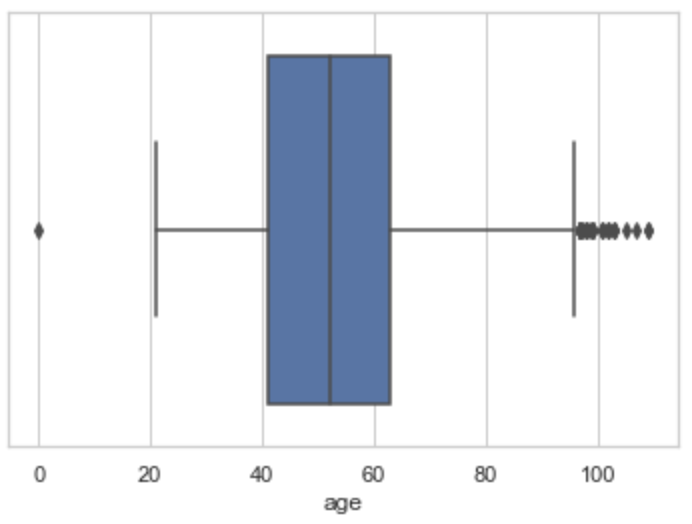
\includegraphics[width=0.40\textwidth]{figures/image5-2.png}}
    \subfigure[对比箱线图]{
    \label{Fig.sub.1}
    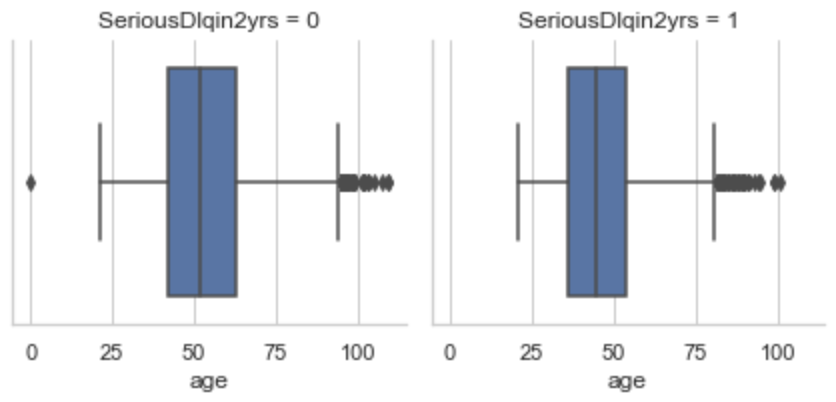
\includegraphics[width=0.55\textwidth]{figures/image5-3.png}}
    \caption{Age}
    \label{Fig.main}
    \end{figure}
    
    \item NumberOfTime30-59DaysPastDueNotWorse表示贷款人逾期30-59天的次数,我们根据数值进行了分布直方图的绘制,发现次数存在大于96次的情况,我们认为这是数据搜集时的偏误,因此我们设置15次为最大的逾期次数,即15次是最大的逾期次数。
     %%image6-----------------(countplot)
    \begin{figure}[H]
    \centering
    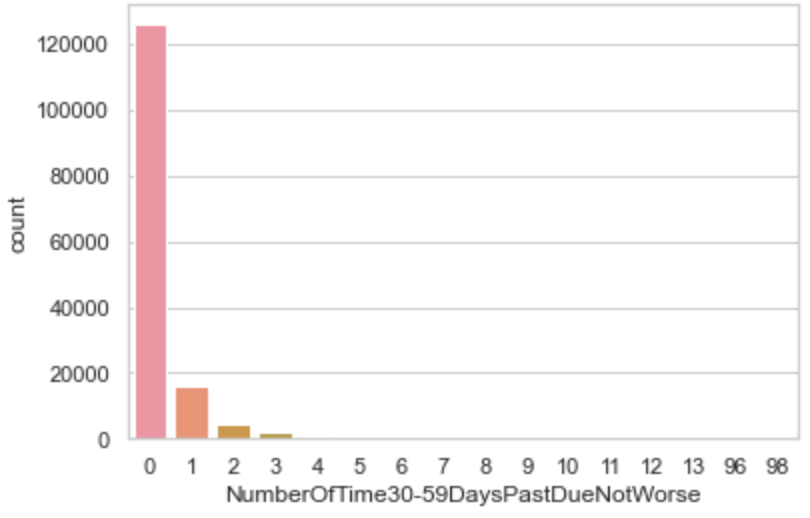
\includegraphics[scale=0.6]{figures/image6.png}\\
    \caption{NumberOfTime30-59DaysPastDueNotWorse直方图}
    \end{figure}
     \item DebtRatio指的是每月的债务支付占每月收入的比率,发现该属性样本之间的差距还是比较大的,并且没有明显的发现该属性于样本标签值之间存在明显的关系,后续可以考虑对该属性进行删除。
      %%image7-----------------(displot)
    \begin{figure}[H]
    \centering
    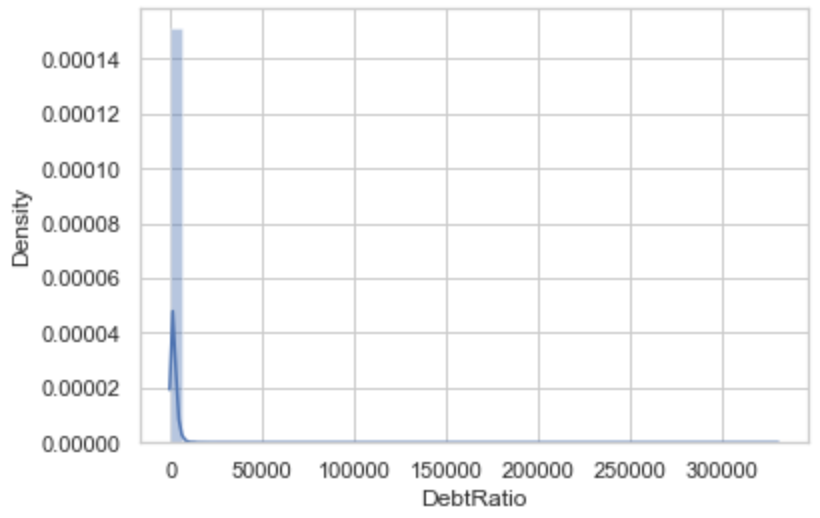
\includegraphics[scale=0.7]{figures/image7.png}\\
    \caption{DebtRatio直方图}
    \end{figure}
      
     \item MonthlyIncome指的是月收入,发现该属性存在较多的缺失值,我们通过筛选发现在训练集中存在1699条语句存在该属性的缺失,因此我们采用平均值对缺失值进行填补。
     \lstinputlisting[language=python]{code/fillna.py}
     \item NumberOfOpenCreditLinesAndLoans指的是未偿还的贷款和信用额度,我们通过绘制对比直方图查看不同标签下未偿还贷款的差异,发现有逾期贷款的贷款者在未偿还贷款的分布上也比较集中。
      %%image8-----------------(displot)
    \begin{figure}[H]
    \centering
    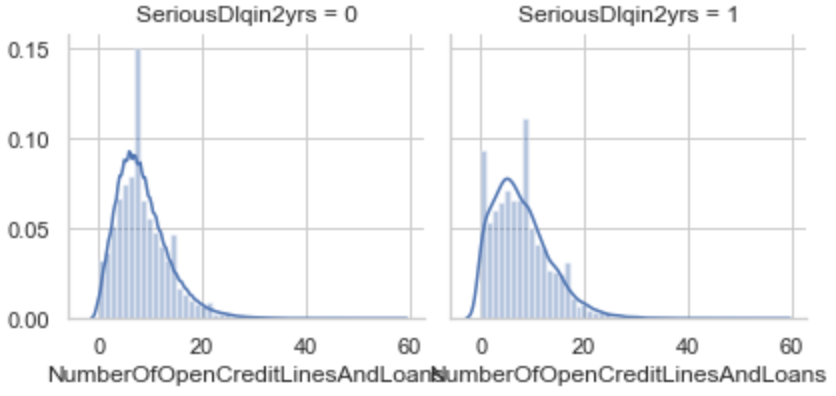
\includegraphics[scale=0.7]{figures/image8.png}\\
    \caption{MonthlyIncome直方图}
    \end{figure}
      \item NumberOfTimes90DaysLate表示的是贷款人逾期90天或者更长的时间次数,我们通过绘制对比数值统计图发现,该属性大的贷款者更容易成为目标样本。同时我们也可以看到一些数据上的问题,我们知道超过90天的次数应该小于等于逾期60-89天的人数,而数据中存在一些不满足的情况,因此同样的,我们将15设置为该属性的最大值,大于的15的值统一替换为15。
       %%image9-----------------(countplot)
    \begin{figure}[H]
    \centering
    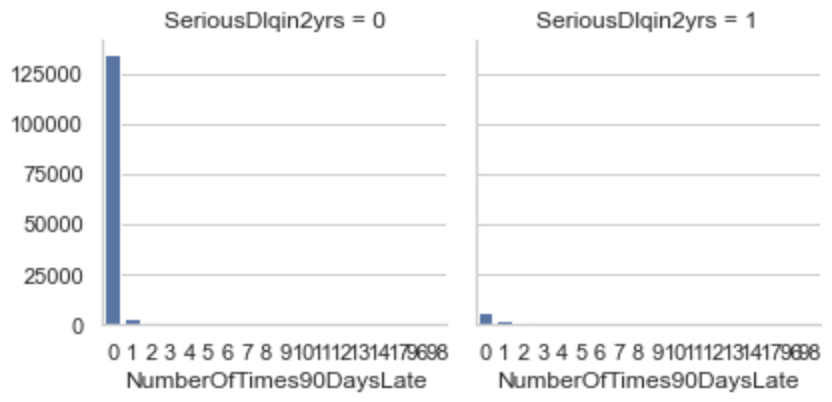
\includegraphics[scale=0.7]{figures/image9.png}\\
    \caption{NumberOfTimes90DaysLate直方图}
    \end{figure}
     \item NumberRealEstateLoansOrLines指的是抵押贷款和房地产贷款的数量,可以看出该属性的类别分布还是存在一定差异的。
      %%image10-----------------(counplot)
    \begin{figure}[H]
    \centering
    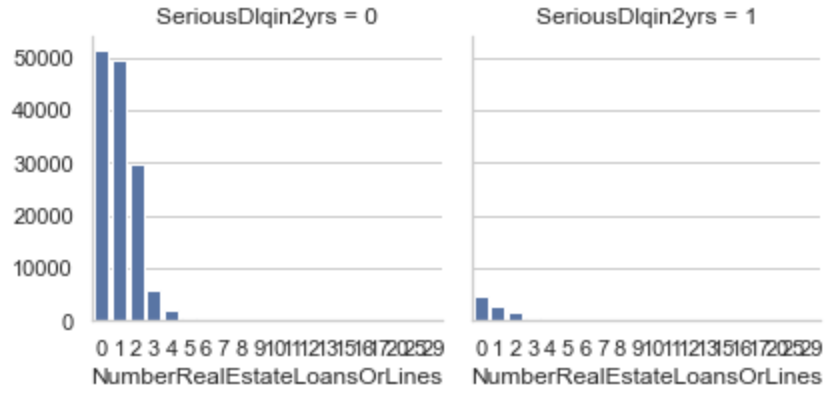
\includegraphics[scale=0.7]{figures/image10.png}\\
    \caption{NumberRealEstateLoanOrLines直方图}
    \end{figure}
     \item NumberOfTime60-89DaysPastDueNotWorse指的是在过去两年中,借款人逾期60-89天但没有恶化的次数,通过对比数值统计图,我们发现,改属性值大的贷款者更容易成为目标样本,并且类似的,我们可以发现一些数据上的问题,也即逾期60-89天的次数应该小于等于逾期30-59天的人数,而数据中有一些情况是不满足的,因此,我们将15设置为该属性的最大值,大于的15的值统一替换为15。
     %%image11-----------------(counplot)
    \begin{figure}[H]
    \centering
    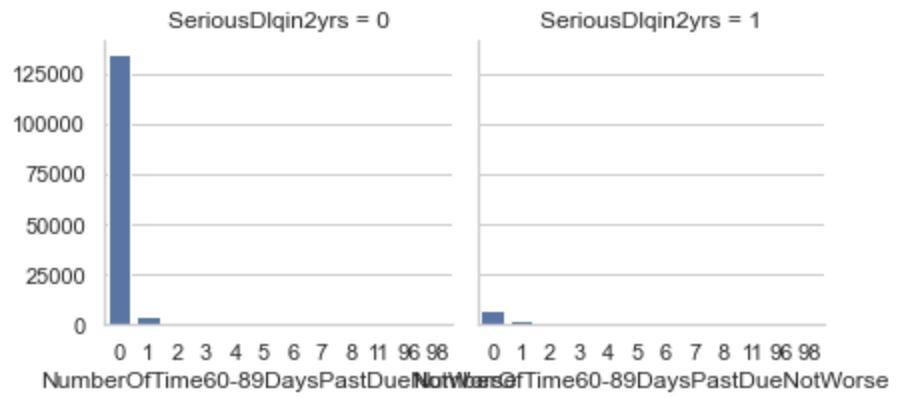
\includegraphics[scale=0.55]{figures/image11.png}\\
    \caption{NumberOfTime60-89DaysPastDueNotWorse直方图}
    \end{figure}
     \item NumberOfDependents指的是家庭成员中受抚养人的数量,通过绘制类别对比的箱线图我们发现类别之间的差异较大,也即更高的赡养负担可能会导致有更多的负债,因此也会有更高的风险,同时我们也发现该数据存在一定确实的情况,同样的我们用平均值填补了缺失。
     %%image12-----------------(boxnplot)
     \begin{figure}[H]
    \centering
    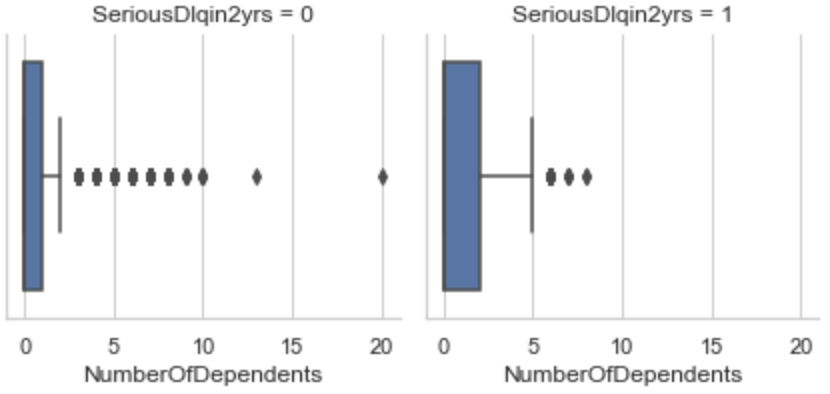
\includegraphics[scale=0.7]{figures/image12.png}\\
    \caption{NumberOfDependdents箱线图}
    \end{figure}
\end{clause}
\subsection{相关性分析}
    为了了解各个属性之间的相关度,我们选用热图来辨识每个属性之间的皮尔逊积相关系数,通过热图我们可以发现SeriousDlqin2yrs和几个逾期天数之间有很大的关系,但是SeriousDlqin2yrs和年龄的关系较小。
    %%image13-----------------(corrplot)
    \begin{figure}[H]
    \centering
    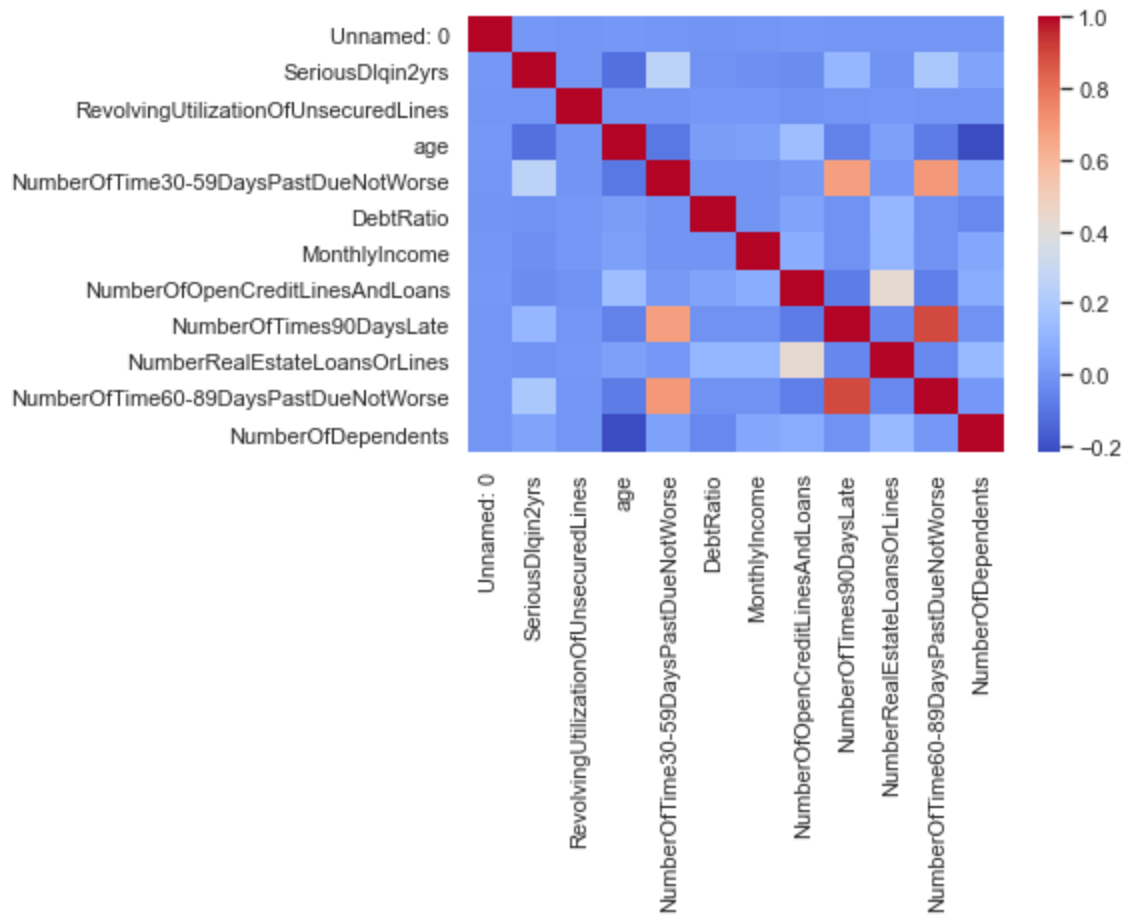
\includegraphics[scale=0.6]{figures/image13.png}\\
    \caption{相关系数图}
    \end{figure}
\section{算法描述与结果分析}
    \subsection{NaiveBayes}
    采用的第一个算法是朴素贝叶斯分类器。对于分类问题:
已知集合: $C=\left\{y_{1}, y_{2}, \ldots, y_{n}\right\}$和$ I=\left\{x_{1}, x_{2}, \ldots, x_{m}, \ldots\right\}$  确定映射规则 $ y=f(x)$使得任意$
x_{i} \in I $有且仅有一个$y_{j} \in C$使得$ y_{j}=f\left(x_{i}\right)$成立。

自然想到的就是贝叶斯分类器。而朴素贝叶斯是一种构建分类器的简单方法。该分类器模型会给问题实例分配用特征值表示的类标签,类标签取自有限集合。它不是训练这种分类器的单一算法,而是一系列基于相同原理的算法:所有朴素贝叶斯分类器都假定样本每个特征与其他特征都不相关。

朴素贝叶斯分类器的一个优势在于只需要根据少量的训练数据估计出必要的参数(变量的均值和方差)。由于变量独立假设,只需要估计各个变量的方法,而不需要确定整个协方差矩阵。


考虑到我们要处理的数据中许多属性是连续数据,故我们采用一般假设,认为这些连续数值为高斯分布。 因此, 对于训练集中某一个连续属性, $x$ 。我们首先对数据根据类别分类,然后计算每个类别中 $x$ 的均值和方差。令 $\mu_{c}$ 表示为 $x$ 在C类上的均值,令 $\sigma_{c}^{2}$ 为 $x$ 在C类上的 方差。在给定类中某个值的概率, $P(x=v \mid c)$, 可以通过将 $v$ 表示为均值为 $\mu_{c}$ 方差为 $\sigma_{c}^{2}$ 正态分布计算出来。也即, $P(x=v \mid c)=\frac{1}{\sqrt{2 \pi \sigma_{c}^{2}}} e^{-\frac{\left(v-\mu_{c}\right)^{2}}{2 \sigma_{c}^{2}}}$ 。但是在大量样本的情形下,另一种方式:离散化连续数值的方法表现更优,因为大量的样本可以学习到数据的分布。由于朴素贝叶斯是一种典型的用到大量样本的方法(越大计算量的模型可以产生越高的分类精确度),所以朴素贝叶斯方法都用到离散化方法,而不是概率分布估计的方法。


    考虑到sklearn已经提供了相关的代码库,供我们直接调用,因此我们可以用如下的语句进行简单的训练:
    \lstinputlisting[language=python]{code/nb.py}
    
    
    得到的ROC曲线如下所示,ROC-AUC score为0.794。
    \begin{figure}[H]
    \centering
    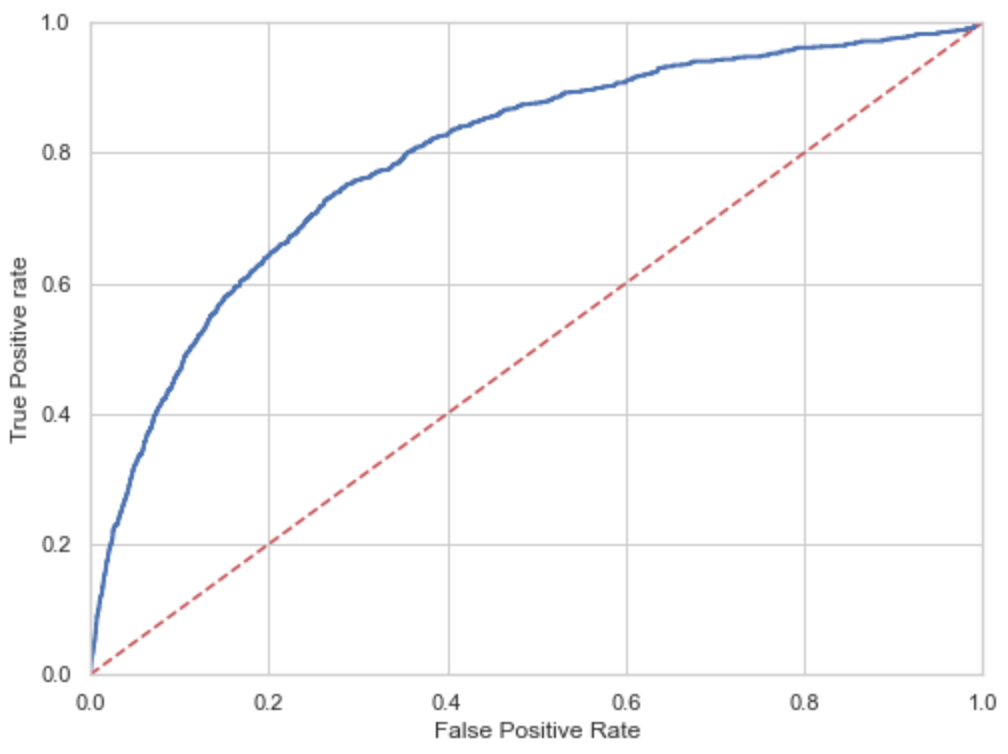
\includegraphics[scale=0.7]{figures/nb.png}\\
    \caption{Naive Bayes}
    \end{figure}
    
    \subsection{RandomForest}
        \subsubsection{(1) Traditional-Random Forest}
        随机森林属于集成学习中bagging算法的延展,Random Forest(RF) 在以决策树作为基学习器构建Bagging集成的基础上,进一步在决策树的训练过程中加入了随机属性的选择。具体来说,传统决策树在选择划分属性时是在当前结点的所有候选属性(假定有d个)中选择一个最优属性;而在RF中,对基决策树的每个结点,先从该结点的候选属性集合中随机选择一个包含k个属性的子集,然后再从这个子集中选择一个最优属性用于划分。抽取的属性数k的选择比较重要,我们一般采用的是$K=log_{2}d$ 。由此,随机森林的基学习器的“多样性”不仅来自样本的扰动,还来自属性的扰动,使得最终集成的泛化能力进一步增强。
        
        随机森林在训练时可以高度并行化,可以有效运行在大数据集上。但是取值划分比较多的特征容易对随机森林的决策产生更大的影响,从而影响拟合的模型效果。同时,随机森林由于对决策树候选划分属性的采样,这样在样本特征维度较高的时候,仍然可以高效的训练模型。但是在某些噪声比较大的样本集上,随机森林容易陷入过拟合。
        
        同样的我们采用sklearn提供的库进行了测试:

        \lstinputlisting[language=python]{code/traditionRF.py}
        
        得到训练的结果如下所示,ROC-AUC值为:0.850,训练时间为416.1s。
        \begin{figure}[H]
        \centering
        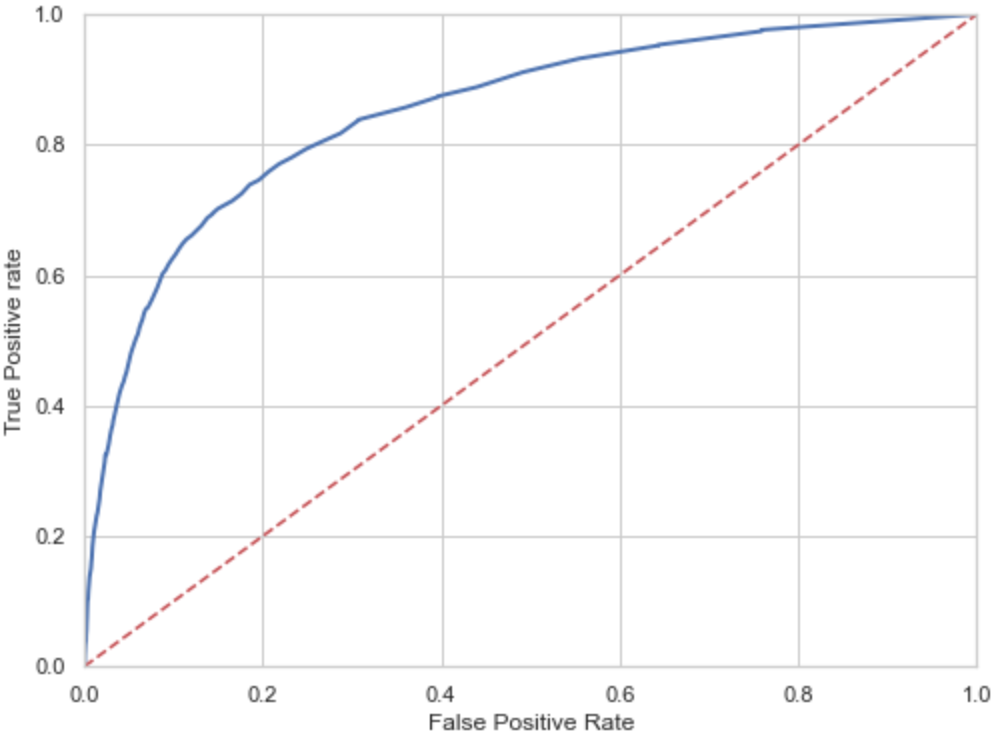
\includegraphics[scale=0.7]{figures/rf1.png}\\
        \caption{Random Forest}
        \end{figure}
        
        
        
        \subsubsection{(2) UnderSampling - Random Forest}
        
        考虑到我们的数据存在类别不均衡的情况(这在前文数据探索性分析时已经发现),我们对传统的随机森林进行了降采样的处理,当训练数据集很大时,它可以通过减少训练数据样本的数量来帮助改善运行时间和存储问题。但是它可能会丢弃有用的信息,并且丢弃的信息对于构建规则分类器可能很重要。另外通过随机欠采样选择的样本可能是有偏差的样本。可能导致实际测试数据集的结果不准确。
        通过引入降采样的模块来跟踪值出现的次数,而后返回降采样后的数值,对重采样以后的数据划分训练集与测试集,然后利用随机森林对重采样之后的数据进行分类,训练过程的代码如下所示:
    
    
    \lstinputlisting[language=python]{code/underRF.py}
    
    得到训练的结果如下所示,ROC-AUC值为:0.867,训练时间为:16.7s。
    \begin{figure}[H]
    \centering
    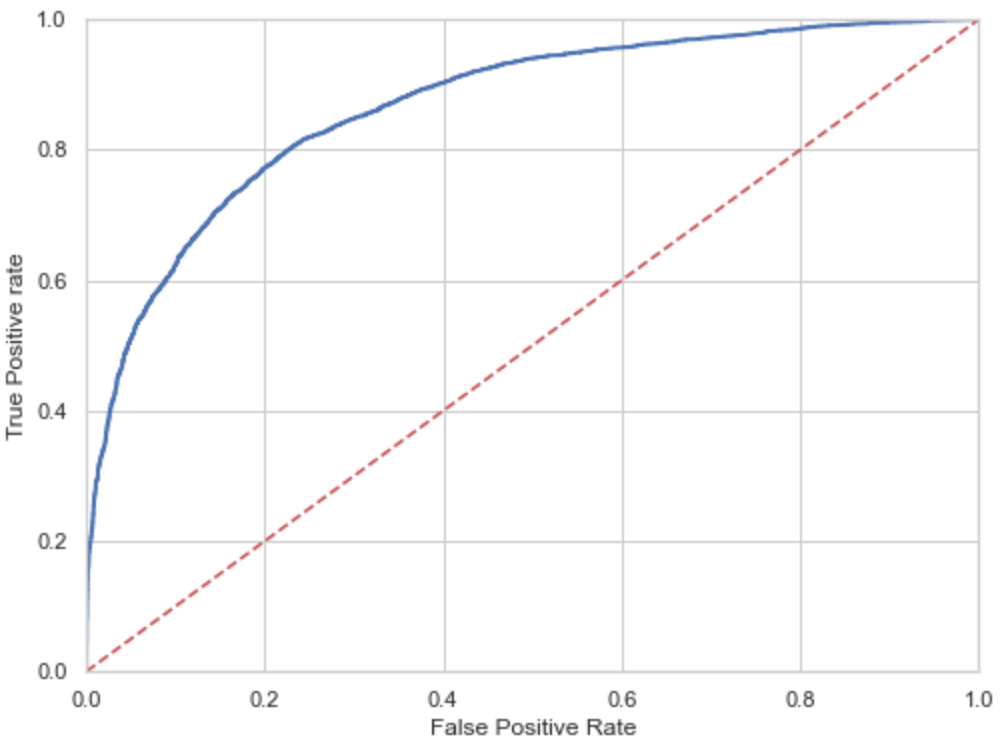
\includegraphics[scale=0.65]{figures/rf2.png}\\
    \caption{UnderSampling - Random Forest}
    \end{figure}
    
    可以发现训练时间相对于原来的Random Forest得到了明显的下降,并且ROC-AUC值得到了略微的提高,再综合训练时间和模型的表现效果来看,采用undersampling的random forest在该数据集上的效果是更优秀的。
    \begin{figure}[H]
    \centering
    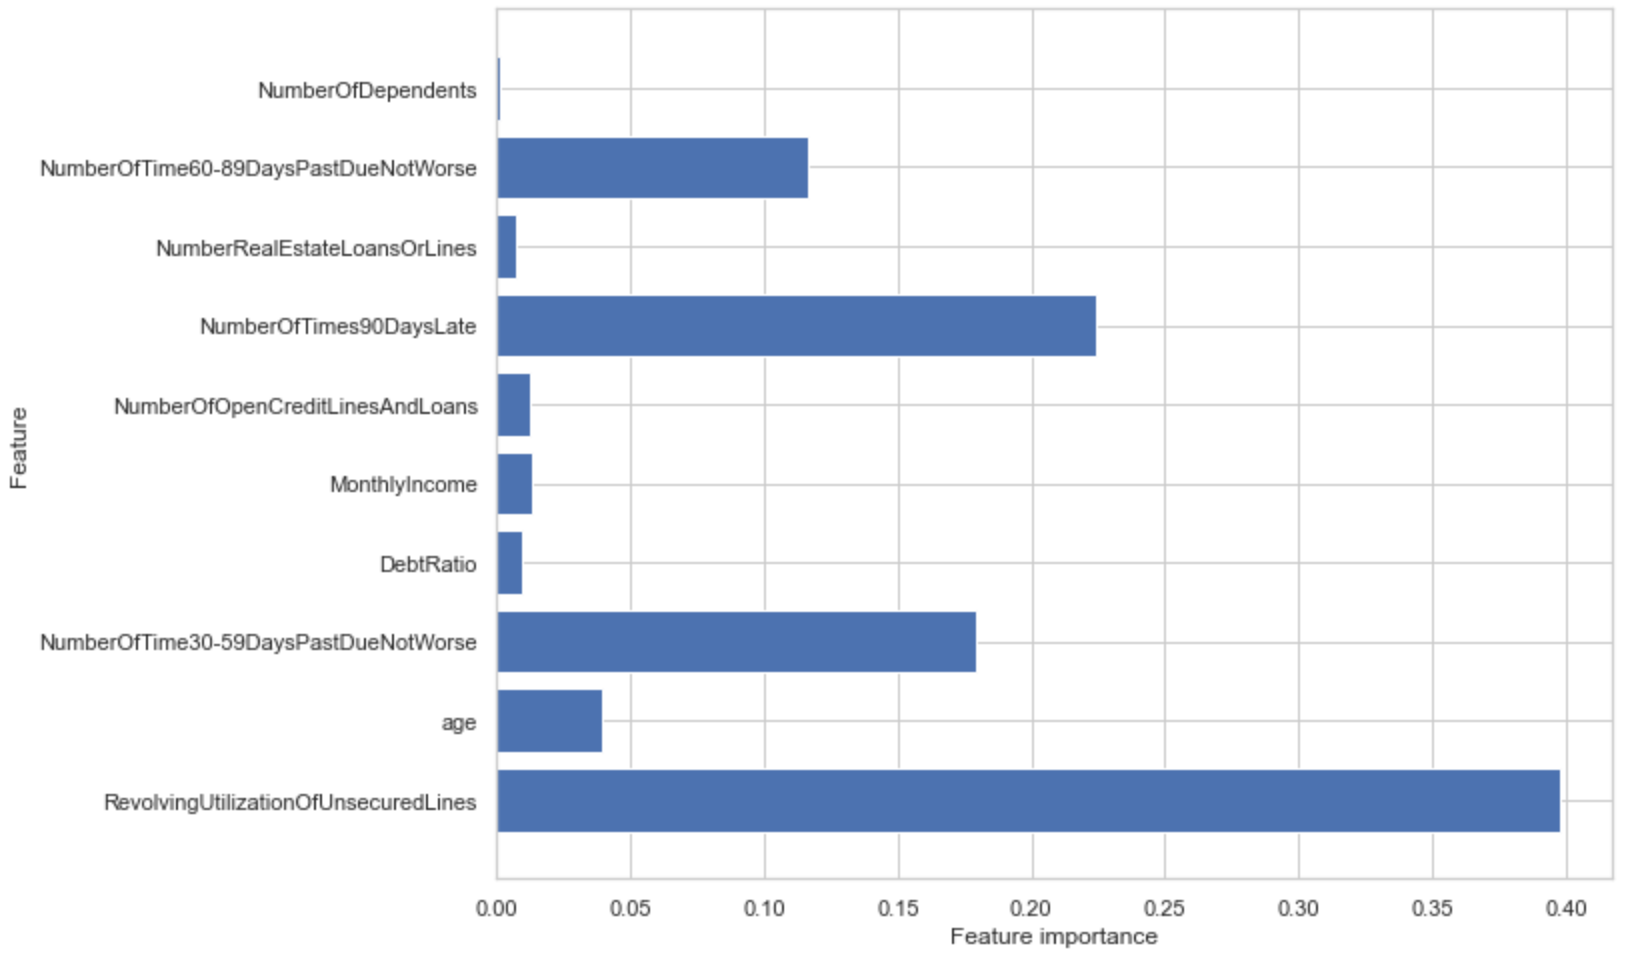
\includegraphics[scale=0.55]{figures/rf3.png}\\
    \caption{UnderSampling - Random Forest对各个特征的重视度}
    \end{figure}
    而后我们可以查看Under sampling对于各个属性的重视程度,发现模型对于RevolvingUtilizationOfUnsecuredLines这一属性是最为看重的,这和我们在数据探索性分析步骤时作出的假设是相一致的,也符合我们的常规认知,也即信用卡和个人信贷余额的总余额越高的贷款者出现逾期信贷的可能性越低。

    
    
    
    
    \subsection{SVM}
        \subsubsection{(1) SVM-RBF}
        我们尝试的第三个算法的带RBF kernel的SVM算法。 RBF核函数可以表示为$k(x,z)=exp(-\rho d(x,z));\rho >0,d(x,z)$是任意距离的度量。采用高斯核函数按一定规律统一改变样本的特征数据得到新的样本,新的样本按新的特征数据能更好的分类,由于新的样本的特征数据与原始样本的特征数据呈一定规律的对应关系,因此根据新的样本的分布及分类情况,得出原始样本的分类情况。主要的方法是得到类似$
x \rightarrow\left(e^{-\gamma|| x-\left.l_{1}\right|^{2} \mid}, e^{-\gamma|| x-\left.l_{2}\right|^{2}}\right)
$的映射,从而衡量样本和样本之间的“相似度”,在一个刻画“相似度”的空间中,让同类样本更好的聚在一起,使得线性不可分的数据线性可分。

可以采用如下的程序实现:
        \lstinputlisting[language=python]{code/SVM.py}
       在运行之后发现采用RBF kernel需要运行的时间为115.6s得到的准确率为:0.931。我们发现运行时间还是较长的,并且我们已经运用sklearn内置的算法包但还是得到了较长的运行时间,因此我们希望能够寻求更高效的算法来提高模型的计算效率。   
        \subsubsection{(2) FPC}
        在查阅相关文献后,我们发现了FPC(Fast Polynomial Kernel Classification)算法,在观察 FPC算法的的设计流程时中,我们发现FPC它提供了一个不同的思路,以避免分类中的maximal margin thoery 。并且FCP使用多项式核的特殊特征,通过ADMM算法而不是 QP 来寻找分类器,而这样做在理论意义上减少了计算负担。我们通过观察FPC的计算流程就可以发现这一点:

    \begin{algorithm}[H]
    \caption{Fast Polynomial kernel Classification(FPC)} %算法的名字
    \hspace*{0.02in} {\bf Input:} %算法的输入, \hspace*{0.02in}用来控制位置,同时利用 \\ 进行换行
    $\text { Input: training samples } D:=\left\{\left(x_{i}, y_{i}\right)\right\}_{i=1}^{m}$\\
    \hspace*{0.02in} {\bf Update:} %算法的结果输出
    \begin{algorithmic}[1]
 
    \For{k=0,1, \ldots,} % For 语句,需要和EndFor对应
      \State  
$u^{k+1}=\left(\beta A^{T} A+\alpha \mathbf{I}_{n}\right)^{-1}\left(\alpha u^{k}+\beta A^{T} v^{k}-A^{T} w^{k}\right) $\\

        %\state
$v^{k+1}=\text { Hinge }_{m \beta}\left(y, A u^{k+1}+\beta^{-1} w^{k}\right)$ \\

       % \state
$w^{k+1}=w^{k}+\beta\left(A u^{k+1}-v^{k+1}\right) $

    \EndFor

    \end{algorithmic}
    \hspace*{0.02in} {\bf End:}
      the first k satisfying  $\left\|p^{k+1}-p^{k}\right\|_{H}^{2}$ < tol with H 
 
    \hspace*{0.02in} {\bf Output:}
     $f_{D, s}(\cdot)=\sum_{j=1}^{n} u_{j}^{\text {output }} K_{s}\left(\eta_{j}, \cdot\right)$
    \end{algorithm}       
        
        可以发现FPC 的优点是减少可调参数,配合以有十分简洁直观的用户友好的设计流程,以及上文提到的ADMM算法降低计算负担。同时阅读论文发现其给出的最优泛化误差保证。
        
        于是我们通过运行如下程序,
        \lstinputlisting[language=matlab]{code/svm-fpc.m}

        得到的training time为5.49s,相比于SVM- RBF确实显著降低了运行时间,但是得到的准确率仅有0.810,这里认为主要是poly-kernel并不太适合处理不平衡且样本个数较多的数据集,但是我们可以从运行时间看到,运行时间是显著提高的,也说明FPC算法的对于SVM的加速是起到作用的。

\section{结果分析与对比}
通过上述三种算法与其对应变形算法的尝试,我们将模型的训练结果进行了简单的对比,如下所示:
\begin{center}
\begin{table*}[htbp]
\centering
  \caption{训练时间与训练结果}
  \label{tab:commands}
  \begin{tabular}{cccccc}
    \toprule
   算法 & Naive Bayes & Traditional-RF& UnderSampling-RF & SVM-RBF & FPC\\
    \midrule

准确率&	0.794(AUC) & 0.850(AUC) & 0.867(AUC)&{\color{blue}{0.931(Accuracy)}}&0.810(Accuracy)\\
运行时间&	\textbf{0.7s}& 416.1s & 16.7s & 115.6s & {\color{red}{5.49s}}\\
Software&Python 3.8 &Python 3.8&Python 3.8&Python 3.8&Matlab 2020b\\



    \bottomrule
  \end{tabular}
\end{table*}
\end{center}  

可以发现在都只是使用简单的CPU的情况下,Naive Bayes Bayes的运行时间是最短的,仅用了0.7s,但是在准确率上的表现并不尽如人意。同时也可以发现RF算法的改进大大缩短了RF算法的运行时间,同时也能够在一定程度上提高模型的准确率。在SVM算法的表现上来看,带有RBF-kernel的SVM算法更适用于解决我们的问题,可以达到0.931的准确率,Poly-kernel在此数据集上的表现并不优秀,主要的原因可能是因为数据集的样本标签是不均衡的,而且数据集本身的样本数较大,特征数相对于样本数来说较小。但是我们可以发现FPC算法能够在很大程度上降低SVM算法的运行时间,并且还是在使用了较为重量的Matlab的情况下。

通过上述实验,我们认为不同的算法都某些角度都能为我们的问题提供一些帮助,但是结合准确率和运行时间来看,UnderSampling的Random Forest 以及 FPC都具有较为不错,也即在权衡运行时间和准确率之后折衷的表现。总体而言,相较于原始的算法,两个改进的算法都具有明显提高的地方。如果不计运行时间的话,只是追求模型的准确率,RBF kernel的SVM算法是实验中所有算法里表现最优的。

\begin{thebibliography}{99}  
\bibitem{ref1}L. Breiman, Random forests, Machnie Learning, 45: 5-32, 2001.
\bibitem{ref2}D. X. Zhou, and K. Jetter, Approximation with polynomial kernels and
SVM classifiers, Adv. Comput. Math., 25: 323-344, 2006.
\bibitem{ref3}Zeng J, Wu M, Lin S B, et al. Fast polynomial kernel classification for massive data[J]. arXiv preprint arXiv:1911.10558, 2019.
\end{thebibliography}
\end{document}
